\documentclass[a4paper,fleqn,12pt]{article}
\usepackage[left=1.5cm, right=2cm]{geometry}
\usepackage[utf8]{inputenc}
\usepackage[sort&compress,numbers]{natbib}
\usepackage{hyperref, graphicx, float, algorithm, algpseudocode, color, xcolor}
\usepackage{amsmath, amsfonts, amssymb, listings, optidef}
\usepackage[cache=false]{minted}
\bibliographystyle{unsrtnat}
\hypersetup{colorlinks=true, linkcolor=blue, filecolor=blue, urlcolor=blue, citecolor=blue}

%%%%% Front matter %%%%%
\title{Dimensionality Reduction Techniques for Subsurface Modeling}
\author{Misael M. Morales, Carlos Torres-Verd\'{i}n, and Michael J. Pyrcz}

\begin{document}
\newcommand*{\vertbar}{\rule[-1ex]{0.5pt}{2.5ex}}
\definecolor{LightGray}{gray}{0.9}
\maketitle
\linenumbers

%%%%% Abstract %%%%%
\section*{Abstract}
Dimensionality reduction is essential for subsurface modeling, where vast datasets with millions of measurements pose computational challenges. Advanced hardware and algorithms have enabled automated rock classification, seismic interpretation, and reservoir simulation, yet high-dimensional data remains a bottleneck. Traditional feature selection helps simplify models, but dimensionality reduction techniques are often required for rapid predictions and enhanced interpretability. Inspired by computer vision, where images are compressed into meaningful features, subsurface modeling benefits from encoding techniques that extract latent representations while preserving critical information. This chapter explores popular dimensionality reduction methods, including singular value decomposition (SVD), principal component analysis (PCA), discrete wavelet transform (DWT), dictionary learning (DL), and deep learning-based autoencoders (AE). These techniques optimize storage, reduce computational costs, and improve predictive accuracy and can be applied to complex workflows such as reservoir simulation, history matching, and geologic modeling. By transforming complex geospatial data into lower-dimensional space, they enhance uncertainty quantification and accelerate machine learning workflows. Hence, the chapter provides insights on different dimensionality reduction techniques for subsurface applications, ensuring robust and scalable modeling for energy resource exploration and development.\\

\noindent {\bf Keywords:} latent space, geologic uncertainty model, spatial data analytics, computer vision

%%%%% Intro %%%%%
\section*{Introduction}
During the last decades, subsurface energy resources have seen immense revolutions with the accelerated developments of hardware and algorithmic technologies to support subsurface modeling \cite{mohammadpoor2020big, latrach2024critical}. For example, rock classification from core measurements and well logs has been automated using clustering and classification algorithms, while reservoir simulation has seen benefits from rapid proxy models for dynamic predictions \cite{raheem2024best, mao2024efficient, morales2024arc, morales2024abc}. In many cases, however, these datasets are composed of thousands or millions of measurements or grid blocks with tens to hundreds of features due to the complexity and uncertainty in subsurface models \cite{Rashid201321, 2021AGUFM.H25O1207S, mao2024cushion}. This makes subsurface modeling a perfect candidate for dimensionality reduction techniques, where hidden patterns and relationships in data can be simplified into lower-dimensional representations for more robust predictions and more interpretable models. 

Supervised machine learning methods, both for regression and classification, can face significant challenges when dealing with large subsurface datasets \cite{tariq2021systematic, sircar2021application}. Several techniques for feature engineering, feature importance, and regularization have been proposed to intelligently reduce problems with a large number of variables to the key ones that have the most effect on the target variable \cite{cai2018feature, zheng2018feature}. However, for cases such as reservoir modeling, seismic modeling, and well log interpretation, a single realization in an uncertainty model can have a large number of features, making dimensionality reduction crucial for rapid machine learning predictions \cite{misra2019machine, bhattacharya2021primer, morales2025anisotropic}. This is a classical problem in the field of computer vision, where a single image can have upward of thousands or millions of pixels, and a single label must be extracted. For subsurface modeling, this translates into interpreting an uncertainty model for example, a multivariate ensemble of subsurface properties (e.g., porosity, permeability, brittleness, total organic content, acoustic impedance), to estimate the recoverable resources in place; or a large 2D or 3D geologic uncertainty model of heterogeneous properties (e.g., porosity, permeability) that can be compressed into a lower-dimensional representation \cite{morales2024stochastic, jiang2023use}.

The main idea behind dimensionality reduction techniques is to compress a dataset, $X$, into a latent representation that retains the majority of the patterns and details in the data, also known as \emph{encoding}, such that,
\begin{equation}
    z=\mathcal{E}(X)
\end{equation}
where $z$ is the latent representation of $X$ and $\mathcal{E}(\cdot)$ is a general encoding operator. The latent representation can then be used for a variety of tasks without the need to use the full-dimensional data given that $z$ contains the majority of patterns and details present in $X$.

Furthermore, the latent representation, $z$, can be decompressed or \emph{decoded} into the original data space using a mirroring operator of the encoder, namely the decoder, $\mathcal{D}(\cdot)$, expressed as,
\begin{equation}
    X'=\mathcal{D}(\mathcal{E}(X))=\mathcal{D}(z).
\end{equation}
The goal is then to minimize the difference between $X$ and $X'$, such that $X\approx X'$, by selecting an optimal latent dimension and encoder and decoder parameters that allow for reduced multicollinearity, reduced storage, and accelerated processing while still retaining the majority of important features in the data \cite{mabadeje2024evaluating, mabadeje2024rigid}. Performing computationally expensive routines, such as reservoir simulation or history matching, with the latent representation instead of the full data space now becomes significantly less computationally expensive and memory intensive, saving computational time and, with the right choice of dimensionality reduction algorithm and latent dimension, sufficiently accurate \cite{morales2025optimal, chen2024assimilation}.

To support the valuable adoption of dimensionality reduction in subsurface modeling, this chapter will focus on the application of several data-driven dimensionality reduction techniques for subsurface modeling, including singular value decomposition (SVD), principal component analysis (PCA), discrete wavelet transform (DWT), dictionary learning (DL), and deep learning-based AutoEncoders (AE). 

\subsection*{Dataset}
To demonstrate the application of different dimensionality reduction techniques in subsurface modeling, a synthetic geologic uncertainty model is used. The dataset consists of an ensemble of Gaussian-distributed log-permeability values simulated using Sequential Gaussian Simulation (SGSIM) in the Stanford Geostatistical Modeling Software (SGeMS) \cite{pyrcz2014geostatistical, pyrcz2024appliedgeostats, remy2009applied}. The values range from $0.69\times10^{-3}$ mD to $6.77\times10^3$ mD. A spherical variogram is used with major and minor values of 90 and 30, respectively. A total of 500 realizations are simulated with a resolution of $128\times128$ for a total of 16,384 parameters, suchat that the original data matrix can be represented as $X\in\mathbb{R}^{500\times128\times128}$. Figure~\ref{fig:geodata} shows the first 15 realizations in the geologic uncertainty ensemble.

\begin{figure}[H]
    \centering
    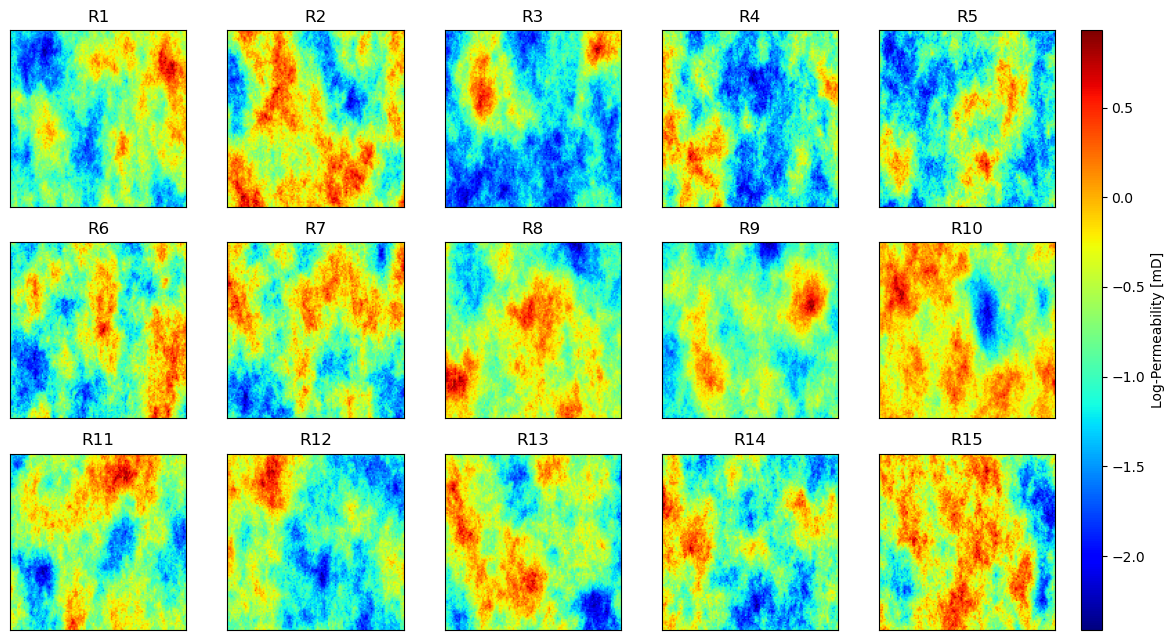
\includegraphics[width=\linewidth]{figures/geodata.png}
    \caption{First 15 realizations (R1-R15) of the geologic uncertainty model depicting log-permeability values.}
    \label{fig:geodata}
\end{figure}

%%%%% SVD %%%%%
\pagebreak
\section*{Singular Value Decomposition}
The singular value decomposition (SVD) is among the most important matrix factorization algorithms of the computing and provides a numerically stable matrix decomposition useful for a wide variety of purposes and applications \cite{klema1980singular, stewart1993early}. Moreover, SVD serves as the underlying algorithm of principal component analysis (PCA), another significant algorithm for dimensionality reduction \cite{wall2003singular, baker2005singular}. While some dimensionality reduction algorithms provide a generic basis for latent, or hidden, low-dimensional representations, such as the fast Fourier transform (FFT) and the discrete wavelet transform (DWT), SVD provides a tailored basis. Tailored basis are extracted directly from the data matrix such that dominant patterns in the data are expressed purely from data, without the addition of expert knowledge or prior information, while generic bases use predetermined functions, such as sines and cosines, to describe the dominant patterns in the data \cite{brunton2022data, jafarpour2009reservoir}. Furthermore, SVD is proved to exist for all matrices, unlike other transformations such as the eigendecomposition, making it flexible and versatile to use with any dataset \cite{golub2013matrix}. 

For subsurface applications, we will focus on image processing or computer vision applications, and where a reservoir model can be described as a matrix with each entry representing a grid block value of a subsurface property, similar to pixels in an image. Let $X$ be our data matrix such that $X\in \mathbb{R}^{n\times m}$ is expressed as, 
\begin{equation}
    X = \left[\begin{array}{cccc}
                        \vertbar & \vertbar &        & \vertbar \\
                        x_{1}    & x_{2}    & \ldots & x_{m}    \\
                        \vertbar & \vertbar &        & \vertbar 
                        \end{array}\right], 
\end{equation}
where each column of $X$ represents a realization of a subsurface uncertainty model, where each realization $x_k\in\mathbb{R}^n$ has $n$ entries representing each pixel or grid block in the model. Often, the number of entries, $n$, (tens of thousands or millions) is much larger than the number of realizations, $m$ (hundreds or thousands). 

The SVD is a matrix decomposition of $X$ such that,
\begin{equation}
    X = U\Sigma V^T ,
\end{equation}
where $U\in\mathbb{R}^{n\times n}$ and $V\in\mathbb{R}^{m\times m}$ are unitary matrices with orthonormal columns, and $\Sigma\in\mathbb{R}^{n\times m}$ is a real non-negative diagonal matrix. The columns of $U$ are called the \emph{left-singular vectors} of $X$ and the rows of $V^T$ are the \emph{right-singular vectors} of $X$. The diagonal entries of $\Sigma$ are called the \emph{singular values} of $X$ and are ordered by magnitude such that the rows and columns of $U$ and $V^T$ represent the strength of importance of the data matrix $X$. Finally, the rank of $X$ is equal to the number of nonzero singular values in $\Sigma$.

In the case of $m\leq n$, $\Sigma$ has at most $m$ nonzero elements in the diagonal and can be expressed as,
\begin{equation}
    \Sigma = \begin{bmatrix} \hat{\Sigma} \\ 0 \end{bmatrix} ,
\end{equation}
where $\hat{\Sigma}$ is the nonzero portion of $\Sigma$. Thus, we can obtain a lower-dimensional representation of $X$ using the so-called \emph{economy} SVD,
\begin{equation}
    X = U\Sigma V^T = 
    \begin{bmatrix} \hat{U} & \hat{U}^\perp \end{bmatrix}
    \begin{bmatrix} \hat{\Sigma} \\ 0 \end{bmatrix}
    V^T ,
\end{equation}
where the columns of $\hat{U}^\perp$ span a complementary and orthogonal vector space of $\hat{U}$.

In the case of a full-rank $\Sigma$, the lower-dimensional representation of $X$ can be obtained by truncation of the SVD. Here, the matrices $\tilde{U}$, $\tilde{\Sigma}$, and $\tilde{V^T}$ represent the truncated versions of the original decomposition matrices up to a chosen singular value such that,
\begin{equation}
    X \approx \tilde{U}\tilde{\Sigma}\tilde{V}^T .
\end{equation}

If $X$ is not full-rank ($rank(X)=r<min(m,n)$), then some singular values of $\Sigma$ are zero. Thus, if we reconstruct the original data matrix using the rank $r$-truncated decomposition then the SVD will be exact, namely,
\begin{equation}
    X = U_r \Sigma_r V_r^T .
\end{equation}

However, for truncation values, $\tau$, smaller than the rank of $X$ (or the number of singular values in $\Sigma$), there are several ways to optimally select $\tau$ \cite{hansen1990truncated}. One such way is the Scree plot, or an elbow plot, of the number of singular values retained against the cumulative sum of the singular values, known as \emph{energy}. Once a truncation value $\tau$ is optimally selected, retaining only the leading rows and columns of $U$, $\Sigma$, and $V^T$ will provide an approximate reconstruction of $X$ and a reduced-dimensional representation of the data matrix.

%%% example
\subsection*{Example}
To perform SVD, we must vectorize the dataset by making each realization a column vector instead of a matrix, namely $X\in\mathbb{R}^{500\times16384}$. Figure~\ref{fig:svd-basis} shows the leading SVD bases obtained for this dataset. Given that the SVD sorts the leading singular values by magnitude, we observe that the first few bases retain information about the large-scale features in the dataset, while the trailing bases retain fine-scale granular details. 

\begin{figure}[H]
    \centering
    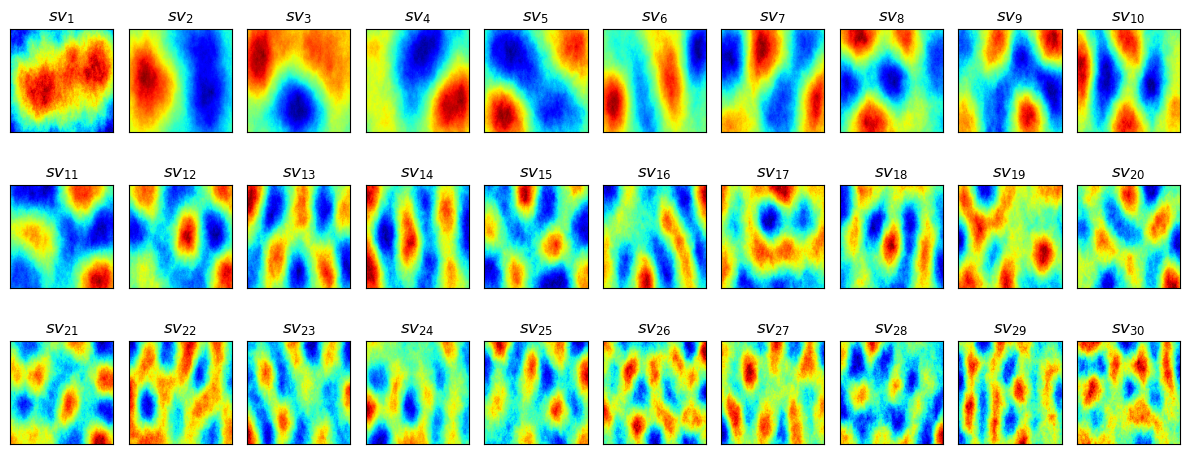
\includegraphics[width=\linewidth]{figures/svd-basis.png}
    \caption{Leading SVD basis (SV$_1$-SV$_{30}$) for geologic uncertainty dataset.}
    \label{fig:svd-basis}
\end{figure}

It is possible to take the SVD of the geologic uncertainty ensemble using different truncation values, $\tau$, since $n\leq m$. The Scree plot in Figure~\ref{fig:svd-scree} shows that by the truncation value $\tau=288$, the singular values account for approximately 80\% of the image energy, and by $\tau=441$, the singular values account for approximately 95\% of the image energy. Figure~\ref{fig:svd-rec} shows the reconstructed images using $k$ singular values at 20\%, 50\%, 80\% and 95\% energy, while Figure~\ref{fig:svd-rec-best} shows that by using only $k=441$ singular values, accounting for 95\% of energy retained here, we are able to accurately reconstruct the ensemble realizations with an average $R^2$=99.27 and structural similarity index measure $SSIM$=98.83. The absolute difference between the true and reconstructed images, expressed as,
\begin{equation}\label{eq:abserr}
    \varepsilon = |\frac{X-X'}{X}| ,
\end{equation}
shows that the the majority of geologic features and important details are retained, while mostly the noise is filtered out and represented as the error or difference between the images. The code for the SVD example can be found in Appendix~\ref{app:svd}.

\begin{figure}[H]
    \centering
    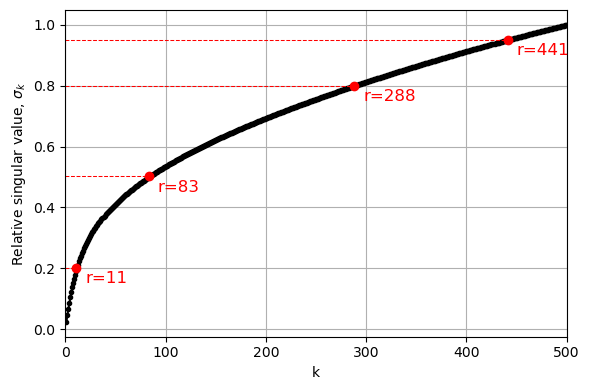
\includegraphics[width=0.5\linewidth]{figures/svd-scree}
    \caption{Cumulative energy in the first $k$ singular values.}
    \label{fig:svd-scree}
\end{figure}

\begin{figure}[H]
    \centering
    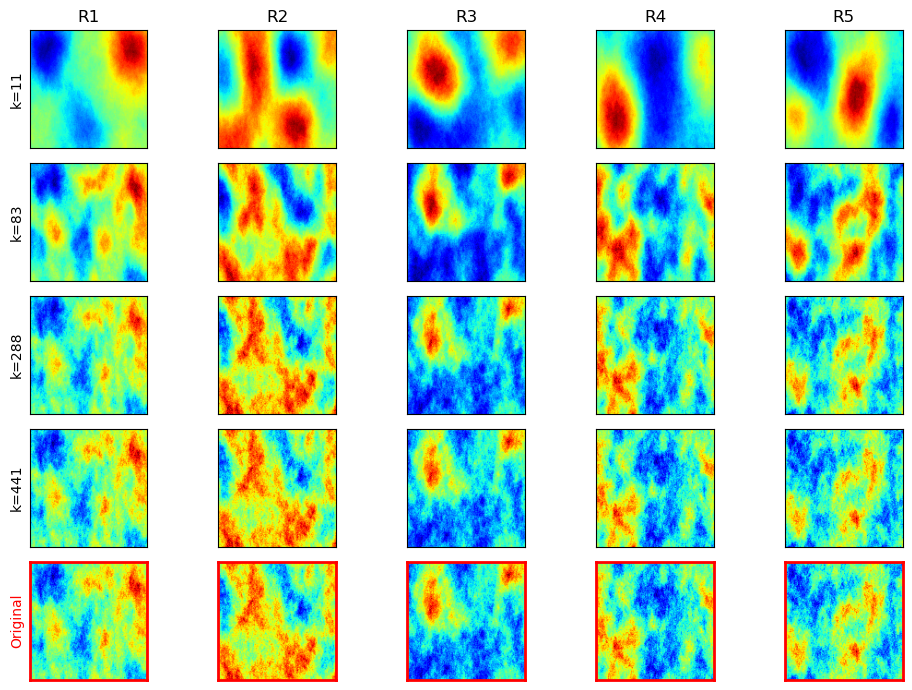
\includegraphics[width=0.85\linewidth]{figures/svd-rec}
    \caption{Reconstructed geologic models using $k$ singular values for the first 5 realizations (R1-R5).}
    \label{fig:svd-rec}
\end{figure}

\begin{figure}[H]
    \centering
    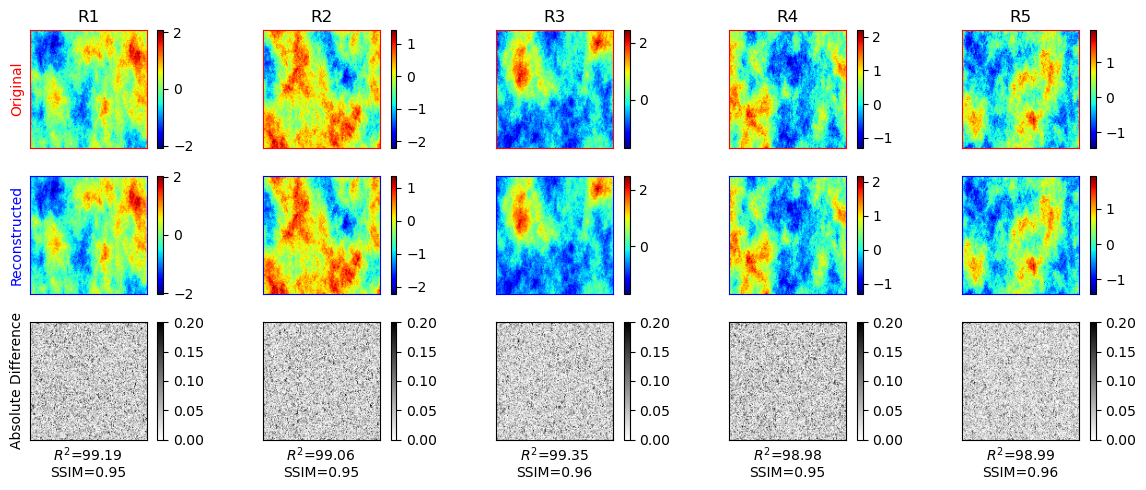
\includegraphics[width=\linewidth]{figures/svd-rec-best.png}
    \caption{Reconstructed images using $k$=441 singular values accounting for 95\% of energy retained for the first 5 realizations (R1-R5). The bottom row shows the absolute difference, calculated using Eq.~\ref{eq:abserr}.}
    \label{fig:svd-rec-best}
\end{figure}

%%%%% PCA %%%%%
\pagebreak
\section*{Principal Component Analysis}

Principal component analysis (PCA) is currently one of the most popular and versatile dimensionality reduction techniques, and it has been widely applied to subsurface modeling \cite{sarma2007new, vo2014new, pyrcz2024appliedml}. Given a data matrix $X\in\mathbb{R}^{n\times m}$, PCA aims to find the best linear subspace in the least-squares sense using the search of rotated orthogonal bases that maximize the variance explained in the first basis vector, followed by the second orthogonal vector, and so on, as shown in Figure~\ref{fig:pca12} \cite{jolliffe2016principal, abdi2010principal}. PCA preprocesses the data by mean subtraction and setting the variance to unity before performing SVD. The resulting coordinate system (principal components) are orthogonal to each other but have maximum correlation with respect to the data measurements. 

Let $B$ be the mean-subtracted matrix such that,
\begin{equation}
    B=X-\overline{X} ,
\end{equation}
and the data covariance matrix be given by,
\begin{equation}
    C=\frac{1}{n-1}B^TB .
\end{equation}
Then the first principal component is given by,
\begin{equation}
    u_1 = \operatorname*{argmax}_{\|u_1\|=1} u_1^TB^TBu_1 ,
\end{equation}
where $T$ represents the transposition operator.

\begin{figure}[H]
    \centering
    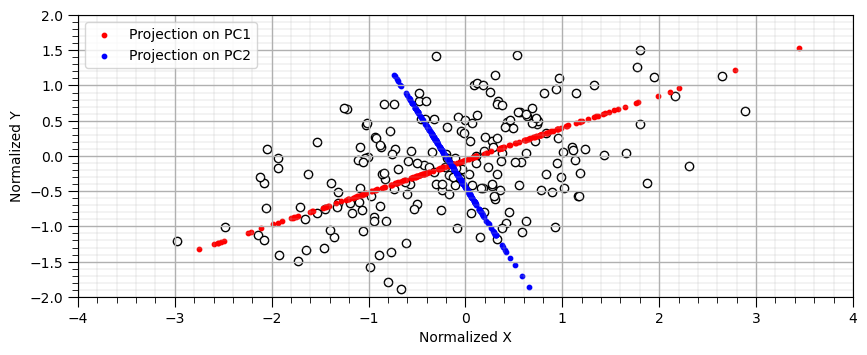
\includegraphics[width=\linewidth]{figures/pca12.png}
    \caption{Random multivariate dataset and PCA projection for the first (red) and second (blue) principal components. The PCA projection is the orthogonal rotation to maximize variance explained in the first principal component and remaining variance in the second principal component.}
    \label{fig:pca12}
\end{figure}

Inherently, $u_1$ is the first eigenvector of the normalized covariance matrix $B^TB$. The maximum number of principal components that can be obtained for a data matrix $X\in\mathbb{R}^{n\times m}$ is given by,
\begin{equation}
    min(m,n-1) ,
\end{equation}
and the remaining principal components can be obtained via de eigendecomposition of $C$, such that,
\begin{equation}
    CV = VD ,
\end{equation}
where $V$ is the matrix whose columns represent the eigenvectors of the covariance matrix $C$, and $D$ is a diagonal matrix of eigenvalues corresponding to each eigenvector of $V$.

PCA converts the set of measurements into a set of linearly uncorrelated features, known as principal components, which are a linear combination of the original features. The principal components form a new orthogonal basis, and the principal component scores, or loadings, provide the linear combination weights. Furthermore, PCA can also be interpreted geometrically as a matrix rotation, where the original measurements are transformed into a linearly independent subspace of orthogonal vectors, namely the principal components, that maximize the variance explained. Similar to SVD, the principal components and their corresponding loadings are ordered by magnitude, where the leading terms account for the largest possible variance explained \cite{esbensen20202}. 

To perform dimensionality reduction on a dataset, we perform truncation and only select $k$ leading principal components to perform the back-transformation. This allows us to reconstruct the back-projected data matrix, $X'$, by maintaining the principal components with the highest variance explained while removing the trailing principal components that represent the nuances or noise in the data.


%%% example
\subsection*{Example}
To perform PCA we must also vectorize the geologic uncertainty dataset by making each realization a column vector instead of a matrix, namely $X\in\mathbb{R}^{500\times16384}$. Similar to SVD, PCA sorts the leading principal components by magnitude. Figure~\ref{fig:pca-basis} shows the leading components. We observe that the first few bases retain information about the large-scale features in the dataset, while the trailing bases retain fine-scale granular details. Figure~\ref{fig:pca-scree} shows that with only $r=234$ PCs, we are able to retain 95\% of the variance explained in the dataset, while using $r=[2,8,36]$ retains 20\%, 50\%, and 36\% of the variance explained in the dataset, respectively.

\begin{figure}[H]
    \centering
    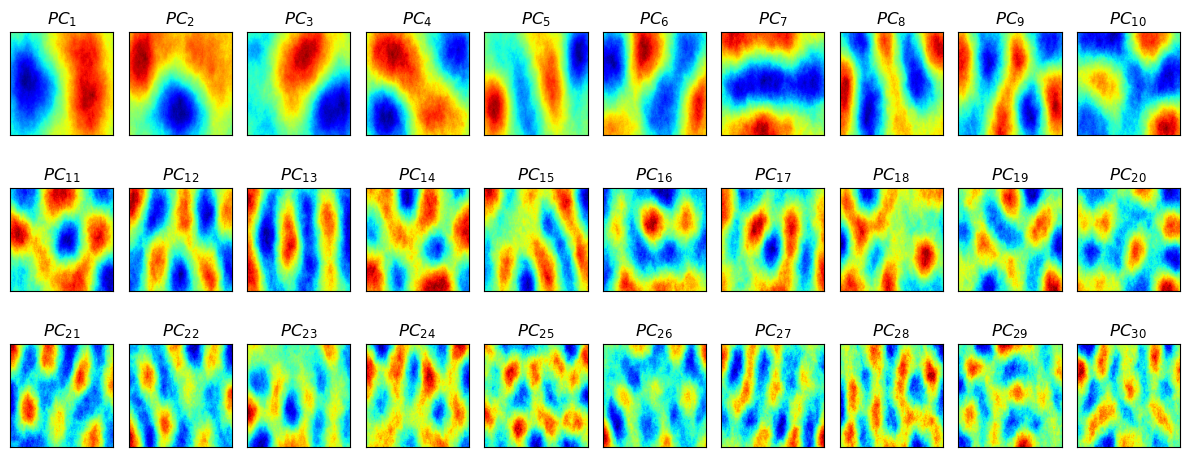
\includegraphics[width=\linewidth]{figures/pca-basis.png}
    \caption{Leading PCA basis (PC$_1$-PC$_{30}$) for geologic uncertainty dataset.}
    \label{fig:pca-basis}
\end{figure}

Figure~\ref{fig:pca-rec} show the reconstructed images using k principal components at 20\%, 50\%, 80\% and 95\% variance explained, while Figure~\ref{fig:pca-rec-best} shows that using only k = 234 principal components, accounting for 95\% of
variance explained, we are able to accurately reconstruct the ensemble realizations with an average $R^2$=95.41 and $SSIM$=92.00. The code for the PCA example can be found in Appendix~\ref{app:pca}.

\begin{figure}[H]
    \centering
    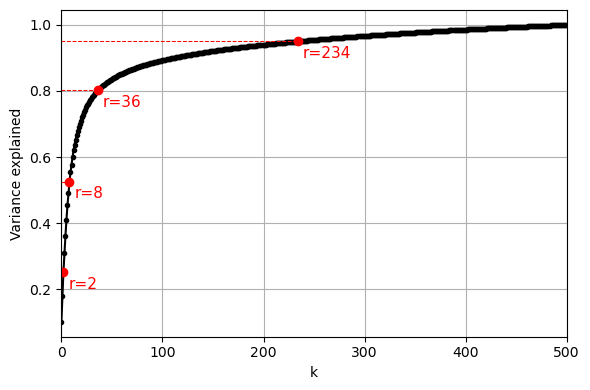
\includegraphics[width=0.55\linewidth]{figures/pca-scree.png}
    \caption{Variance explained against the first $k$ principal components.}
    \label{fig:pca-scree}
\end{figure}

\begin{figure}[H]
    \centering
    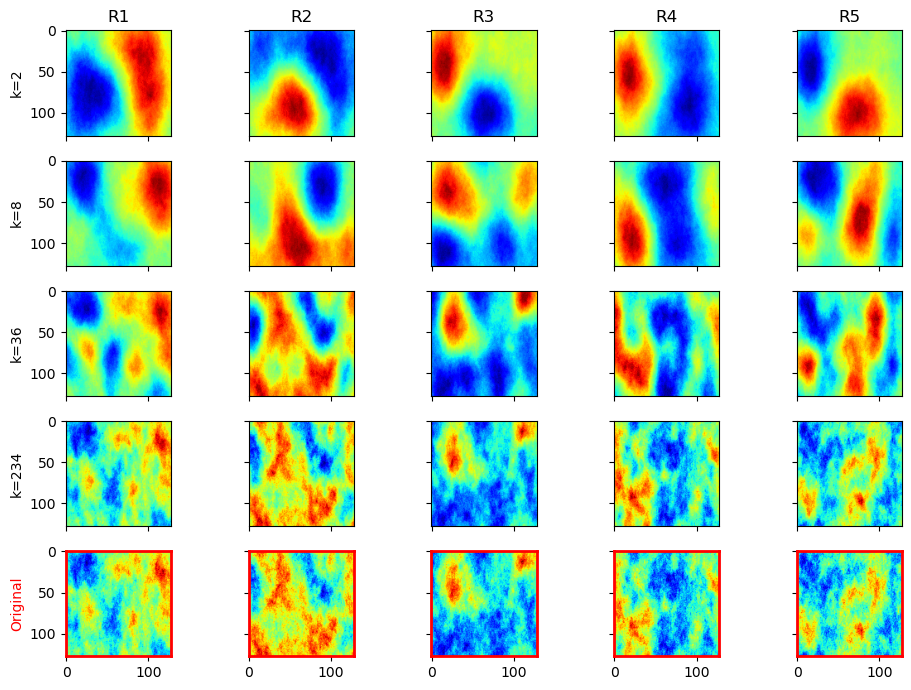
\includegraphics[width=\linewidth]{figures/pca-rec.png}
    \caption{Reconstructed geologic models using $k$ principal components for the first 5 realizations (R1-R5).}
    \label{fig:pca-rec}
\end{figure}

\begin{figure}[H]
    \centering
    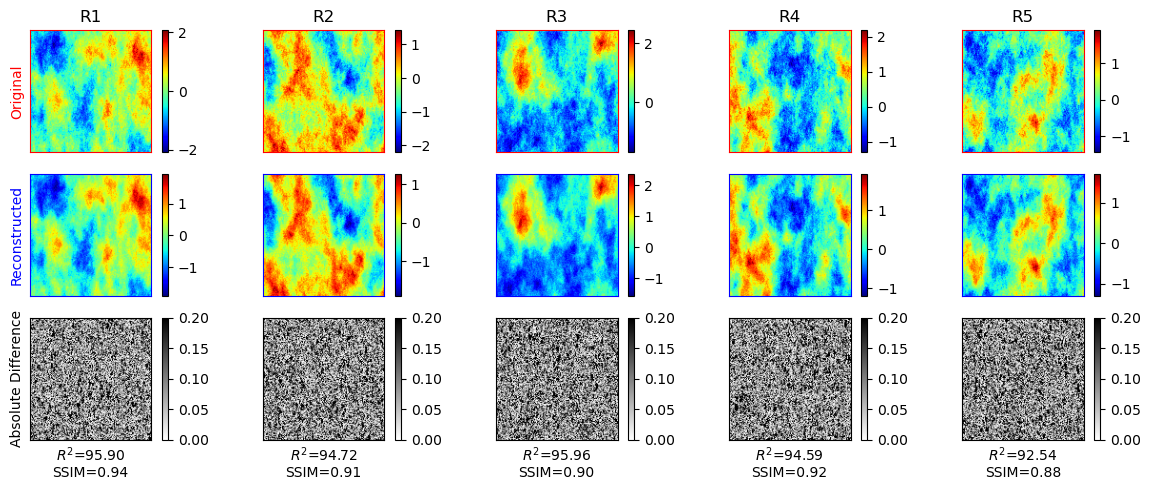
\includegraphics[width=\linewidth]{figures/pca-rec-best.png}
    \caption{Reconstructed images using $k$=234 principal comonents accounting for 95\% of variance explained for the first 5 realizations (R1-R5). The bottom row shows the absolute difference, calculated using Eq.~\ref{eq:abserr}.}
    \label{fig:pca-rec-best}
\end{figure}

%%%%% DWT %%%%%
\pagebreak
\section*{Discrete Wavelet Transform}

To explain the discrete wavelet transform, one must first take a look at the Fourier transform. The Fourier transform is a central topic in physics and engineering, involving a transformation of equations into a simple basis to simplify and decouple equations and make computations and analysis more efficient \cite{duhamel1990fast, li2020fourier}. The main idea behind the Fourier transform is to decompose a signal into a set of sine and cosine functions with increasing frequencies to provide an orthogonal basis for the space of solutions to an equation \cite{iorio2001fourier}. Unlike SVD and PCA, where the set of orthogonal bases are \emph{tailored} to the data, the Fourier transform provides a \emph{generic} basis (sines and cosines) to parameterize any data space into frequency and phase \cite{brunton2022data}.

Mathematically, the Fourier transform is expressed as
\begin{equation}
    f(x) = \frac{a_0}{2} + 
    \sum_{k=1}^\infty [a_k cos(\frac{k\pi x}{L}) + b_k sin(\frac{k\pi x}{L})] 
    = \sum_{k=-\infty}^{\infty} c_k e^{\frac{ik\pi x}{L}} ,
\end{equation}
where $a_k$ and $b_k$ are the sine and cosine coefficients, respectively, $L$ is the domain range such that $x\in[-L,L]$, and $k$ is the frequency.

Computationally, the Fourier transform of a data matrix can be computed using the Fast Fourier Transform \cite{cooley1969fast, nussbaumer1982fast}. This classical algorithm has become ubiquitous in all fields of science and engineering, allowing for rapid image and audio compression and other applications. However, the Fourier transform suffers from localization and loss of resolution, especially in time-frequency analysis \cite{susrutha2019analysis}. Wavelets and the Discrete Wavelet transform (DWT) become the candidate solution for more complex problems.

DWT is based on the Fourier transform, but extends the transformation to a more general orthogonal basis and exploits multi-resolution decompositions by enabling different time and frequency scales, namely the decomposition levels \cite{heil1989continuous, edwards1991discrete}. This is particularly useful for decomposing complex measurements, especially for image and video decomposition and compression \cite{othman2020applications}. The principal idea behind DWT is to start with a generating function, $\psi(t)$, also known as the \emph{mother} wavelet, and generate a family of scaled and translated versions of the function, such that,
\begin{equation}
    \psi_{a,b}(t) = \frac{1}{\sqrt a}\psi(\frac{t-b}{a}),
\end{equation}
where $a$ and $b$ are learnable parameters representing the scale and translation of the function $\psi$, respectively. Typically, the generating wavelet is selected to be an orthogonal function to provide a hierarchical basis. Therefore, any dataset or function $X=f(t)$ can be descibed as 
\begin{equation}
    X = \sum_{k=-\infty}^{\infty}a_k\phi(t) + \sum_{k=-\infty}^{\infty}\sum_{j=0}^{\infty}b_{j,k}\psi(t) ,
\end{equation}
where $\phi$ is a scaling function, $\psi$ is the general wavelet, and $a$ and $b$ are the scaling and translation parameters, respectively.

For a 2D image, a level 1 DWT decomposition divides the data matrix into two discrete components, namely the approximation and details. A filter bank, or cascading set of high-pass and low-pass filters, is applied to the data matrix such that the first set obtains a low-pass horizontal filter (L) and a high-pass horizontal filter (H). Then each sub-image is filtered vertically using the low-pass and high-pass filter to obtain LL, HL, LH, and HH, respectively, also referred to as the approximate ($A$), horizontal ($H$), vertical ($V$), and diagonal ($D$) coefficients. The level 1 DWT coefficient matrix can then be represented as,
\begin{equation}\label{eq:dwt-matrix}
    X = \left[\begin{array}{cccc} A & H \\ V & D \end{array}\right] .
\end{equation}

% example
\subsection*{Example}
The first step to perform DWT is to select hyperparameters, namely the mother wavelet and the number of decomposition levels. Here, we will use only 1 decomposition level and the Haar wavelet, which provides the orthogonal basis needed for the decomposition. Since DWT provides a multi-resoltuion orthogonal basis in two-dimensional space, there is no need to vectorize the data matrix $X\in\mathbb{R}^{500\times128\times128}$. Figure~\ref{fig:dwt-basis} shows the coefficients in the DWT decomposition for the first few realizations of our geologic uncertainty model dataset. Figure~\ref{fig:dwt-scree} shows the structural similarity index measure ($SSIM$) of the reconstructed versus true images in the ensemble as a function of the percent of DWT coefficients retained. 

\begin{figure}[H]
    \centering
    \includegraphics[width=\linewidth]{figures/dwt-basis-new.png}
    \caption{DWT basis, or wavelet coefficients (WC$_1$-WC$_{30}$), for geologic uncertainty dataset. The top left quadrant represents the approximate (A) coefficients, the top right quadrant represents the horizontal coefficients (H), the bottom left quadrant represents the vertical (V) coefficients, and the bottom right quadrant represents the diagonal coefficients (D), as expressed in Eq.~\ref{eq:dwt-matrix}.}
    \label{fig:dwt-basis}
\end{figure}

To obtain a latent representation of reduced-dimensions from the DWT projection, we must truncate the trailing coefficients based on their magnitudes. We observe that by retaining only 5\% of the DWT coefficients, we obtain a reconstruction with $SSIM=46.2$, while retaining 20\% of the DWT coefficients already provides a reconstruction with $SSIM=94.7$, and retaining 50\% of the DWT coefficients provides an almost lossless reconstruction with $SSIM=99.36$. Figure~\ref{fig:dwt-rec} shows the reconstructed images from the geologic uncertainty ensemble using 5\%, 20\%, 50\% and 80\% of DWT coefficients, while Figure~\ref{fig:dwt-rec-best} shows that using only 50\% of the DWT coefficients, we are able to obtain an accurate reconstruction with $SSIM=99.36$, $R^2=99.26$, and $MSE=0.027$. The code for the DWT example can be found in Appendix~\ref{app:dwt}.

\begin{figure}[H]
    \centering
    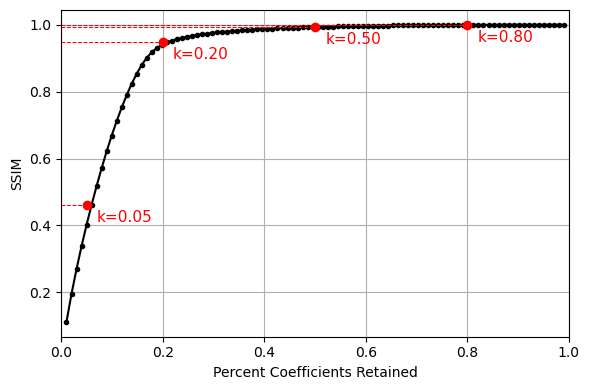
\includegraphics[width=0.5\linewidth]{figures/dwt-scree.png}
    \caption{SSIM by number of DWT coefficients retained.}
    \label{fig:dwt-scree}
\end{figure}


\begin{figure}[H]
    \centering
    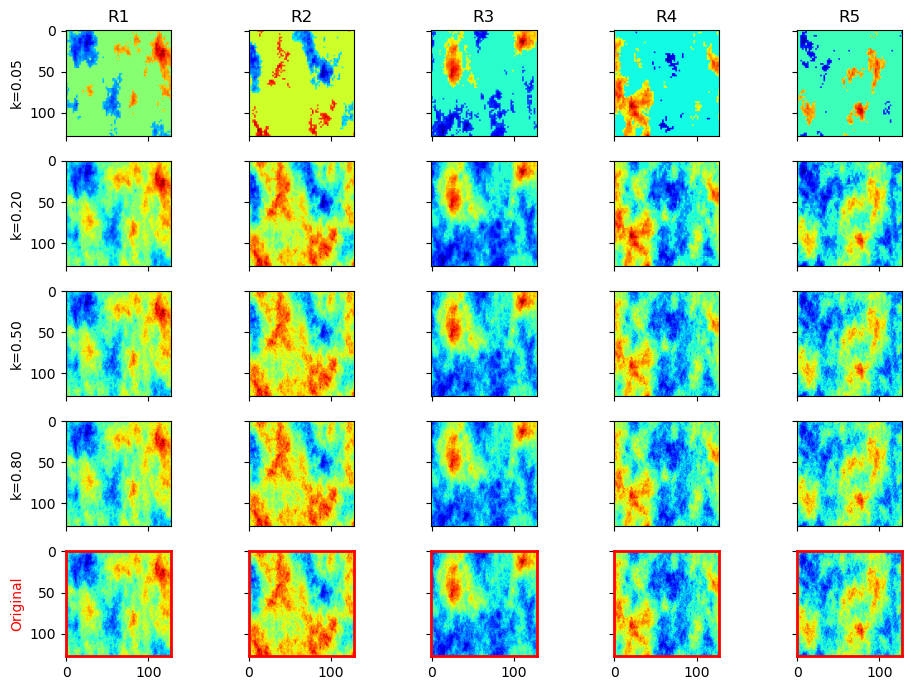
\includegraphics[width=\linewidth]{figures/dwt-rec.png}
    \caption{Reconstructed geologic models by retaining k=\{5, 20, 50, 80\}\% of DWT coefficients for the first 5 realizations (R1-R5).}
    \label{fig:dwt-rec}
\end{figure}

\begin{figure}[H]
    \centering
    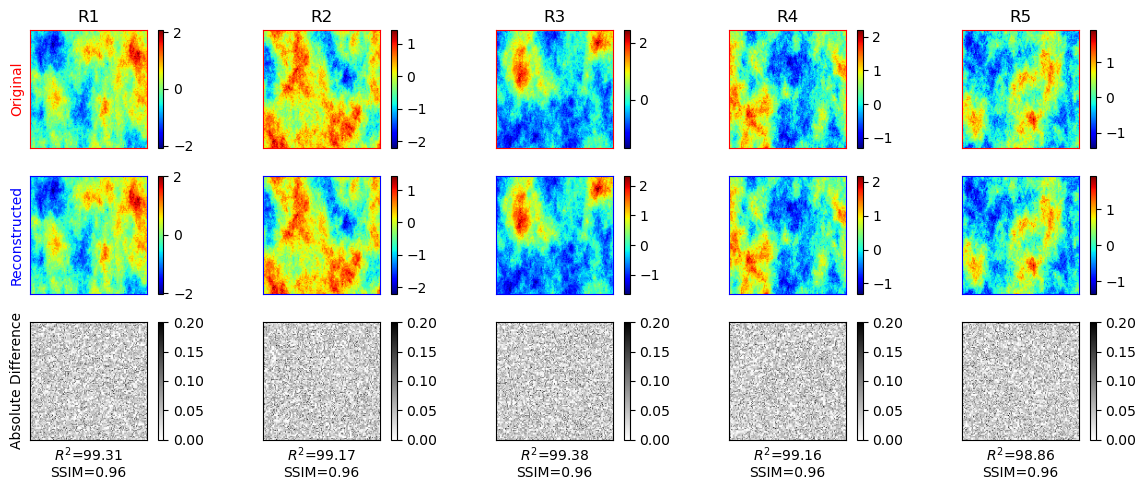
\includegraphics[width=\linewidth]{figures/dwt-rec-best.png}
    \caption{Reconstructed images using k=50\% DWT coefficients accounting for 99\% SSIM for the first 5 realizations (R1-R5). The bottom row shows the absolute difference, calculated using Eq.~\ref{eq:abserr}.}
    \label{fig:dwt-rec-best}
\end{figure}

%%%%% DL %%%%%
\pagebreak
\section*{Dictionary Learning}
Dictionary Learning (DL) is a sparsity-promoting dimensionality reduction method that aims to find a sparse representation of the data matrix from a linear combination of basic elements \cite{tovsic2011dictionary, mairal2008supervised}. The basic elements, known as \emph{atoms} or \emph{words}, need not to be orthogonal, as the \emph{dictionary} of atoms can be overcomplete (more atoms than realizations) or undercomplete (less atoms than realizations). For dimensionality reduction purposes, we will focus on undercomplete dictionaries where the data signal can be represented with a linear combination of a limited number of atoms.

Similar to PCA and SVD, dictionary learning provides a \emph{tailored} basis for the data, where the atoms are not generic, but rather, learned from the samples directly. DL takes advantage of the fact that images can often be represented as sparse signals, meaning that a set of images can be represented as a linear combination of basic images, namely the atoms. The atoms can be members of the ensemble or new realizations that combine features from the general population. The data matrix, $X$, is approximated by the dictionary, $D$, and the sparse code, $S$, such that,
\begin{equation}
    X \approx DS .
\end{equation}
Because the dictionary is not a unique parameterization, this becomes a minimization problem such that
\begin{mini}
  {}{\|X-DS\|^2_F}{}{}
  \addConstraint{\|s_i\|_0 \leq K}
  \addConstraint{\|d_i\|_2^2 \leq 1}
\end{mini}
where $K$ is the sparsity level, $d_i$ are the atoms in the dictionary, and $\|\cdot\|_F$ is the Frobenius norm. However, the $\ell_0$-norm is a non-convex and discontinuous function, making the problem $NP$-hard and intractable. Therefore, the solution is obtained using a relaxation term, or regularization, such that the minimization becomes,
\begin{equation}
    \operatorname*{min}_{D,S} \sum_{i=1}^{K} \|X-DS\|_F^2 + \lambda\|s_i\|_0 .
\end{equation}
This formulation still leads to a sparsity-promoting solution using a compressed sensing technique, given that $S$ is sufficiently sparse, $D$ is orthonormal, and $X$ contains sufficient measurements \cite{kreutz2003dictionary, liu2013learning}. The compressed sensing solution of the underdetermined problem now forces $D$ to be orthonormal under the optimal sparsity constraint. The choice of the regularization hyperparameter, $\lambda$, must also be carefully considered. 

The most common approach to solve this minimization problem is the $k$-SVD algorithm, which is a generalization of the $k$-Means algorithm with iterative SVD to update the atoms of dictionary. This two-step solution aims to find the optimal sparse coding, $S$, followed by updating the dictionary, $D$, to encode each element in the data matrix by a linear combination of not more than $K$ atoms. 

% example
\subsection*{Example}
Dictionary Learning (DL) can be efficiently applied for dimensionality reduction of image ensembles such as our geologic uncertainty example. First, we construct a complete dictionary (500 atoms) to observe the sparse representations obtained by DL, as shown in Figure~\ref{fig:dl-basis}. However, since most images can be represented as a linear combination of sparse signals, we can construct an undercomplete dictionary to parameterize the data. The atoms in the dictionary are not necessarily ordered by magnitude or energy preserved, but are altogether a sparse representation of the data matrix. Figure~\ref{fig:dl-scree} shows $SSIM$ of the of the reconstructed data matrix against the number of atoms in the dictionary used to reconstruct. We observe that $k=191$ atoms provide an $SSIM=0.50$, while using $k=426$ and $k=491$ atoms gives $SSIM=0.8$ and $SSIM=0.95$, respectively.

\begin{figure}[H]
    \centering
    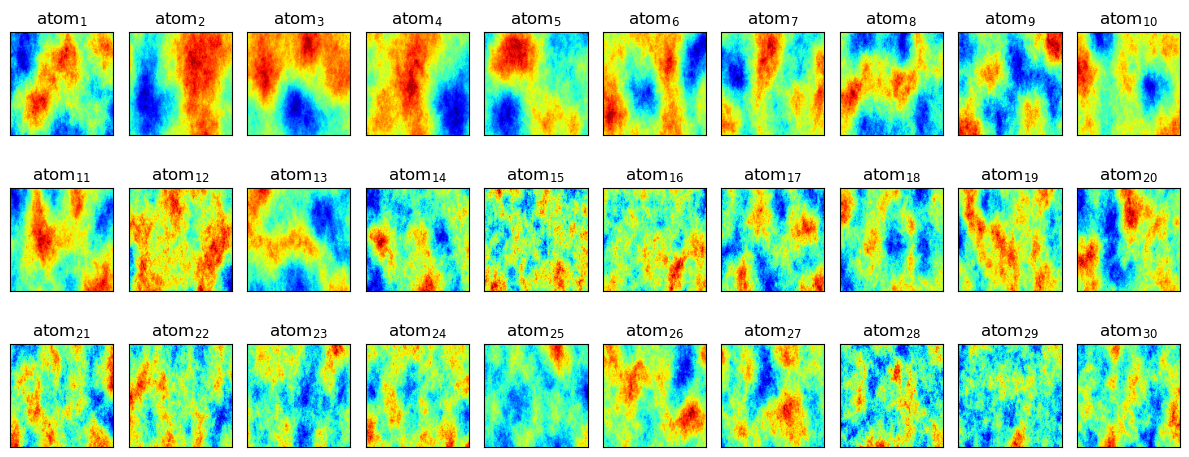
\includegraphics[width=\linewidth]{figures/dl-basis.png}
    \caption{Dictionary atoms or basic images (atom$_1$-atom$_{30}$) for geologic uncertainty dataset.}
    \label{fig:dl-basis}
\end{figure}

Figure~\ref{fig:dl-rec} shows the reconstructed image using $k=16$, $k=191$, $k=426$, and $k=491$ atoms, representing a reconstruction $SSIM$ of 0.20, 0.50, 0.80, and 0.95, respectively. We observe that using only 16 atoms, most reconstructions are not able to capture the patterns in the first few realizations of the ensemble. However, with 191 atoms, the main patterns in the images are reconstructed, and with 426 atoms we have almost lossless reconstructions. Figure~\ref{fig:dl-rec-best} shows the true and reconstructed samples using $k=426$ atoms with an average $SSIM=0.80$ and $R^2=0.97$. The code for the DL example can be found in Appendix~\ref{app:dl}.

\begin{figure}[H]
    \centering
    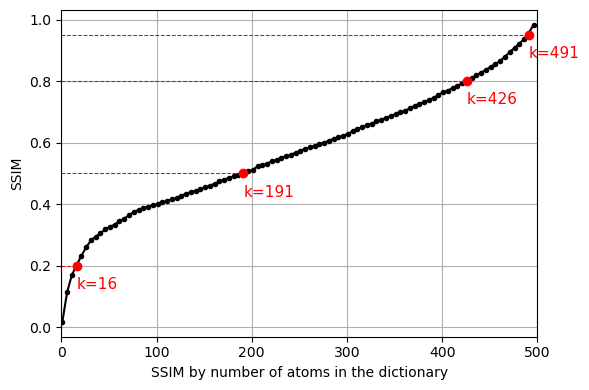
\includegraphics[width=0.5\linewidth]{figures/dl-scree.png}
    \caption{SSIM by number of dictionary atoms retained.}
    \label{fig:dl-scree}
\end{figure}

\begin{figure}[H]
    \centering
    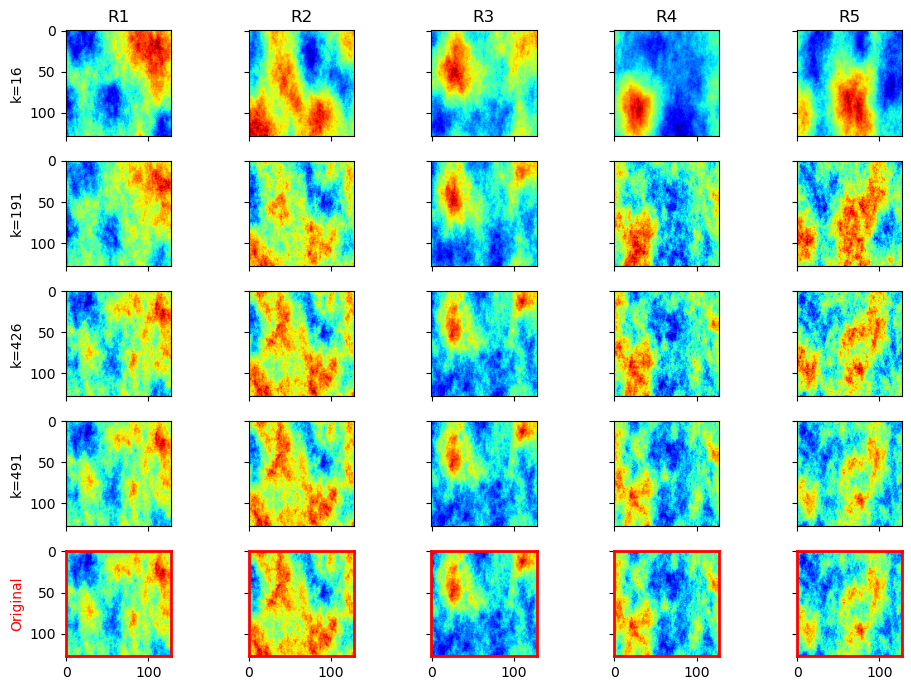
\includegraphics[width=\linewidth]{figures/dl-rec.png}
    \caption{Reconstructed geologic models by retaining k dictionary atoms for the first 5 realizations (R1-R5).}
    \label{fig:dl-rec}
\end{figure}

\begin{figure}[H]
    \centering
    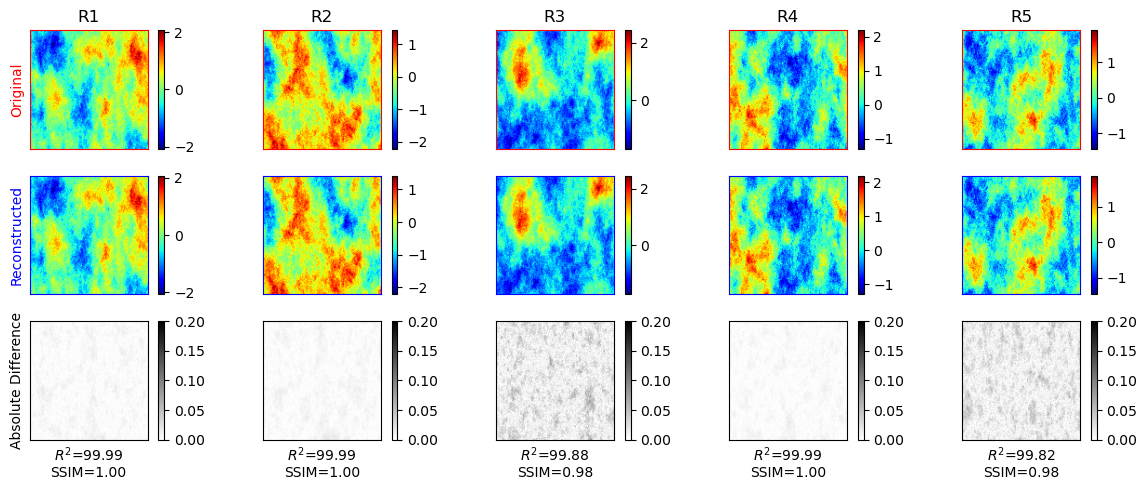
\includegraphics[width=\linewidth]{figures/dl-rec-best.png}
    \caption{Reconstructed images using k=426 dictionary atoms accounting for 80\% SSIM for the first 5 realizations (R1-R5). The bottom row shows the absolute difference, calculated using Eq.~\ref{eq:abserr}.}
    \label{fig:dl-rec-best}
\end{figure}

%%%%% AE %%%%%
\pagebreak
\section*{AutoEncoders}
Over the last decade, neural networks have gained significant popularity in all applications of science and engineering \cite{goodfellow2016deep, zhang2022application}. Advances in computational power and data availability make neural networks candidate methods for great many types of complex problems including computer vision. In general, neural networks can be posed as an optimization function over a functional composition such that,
\begin{equation}
    \operatorname*{argmin}_{A_j} f_M (A_m, \dots, f_2(A_2, f_1(A_1, x))\dots)+\lambda g(A_j) ,
\end{equation}
where $A_k$ represents the matrix of weights between the layers $k$ and $k+1$ of the network, $f$ is a nonlinear operator, and $g(\cdot)$ and $\lambda$ are a regularization function and weight, respectively. The optimization problem quickly becomes a severely ill-posed problem due to the large numbers of parameters, $A_k$, and is typically solved by stochastic gradient descent algorithms and backpropagation \cite{bottou1991stochastic}. 

Convolutional Neural Networks (CNNs) are a specialized type of neural network architecture designed for processing data that has a known grid-like topology, such as images \cite{li2021survey}. Furthermore, they provide inherent regularization properties through the extraction of smaller pixel subsets and simpler patterns from images. The convolution operator extracts features from overlapping receptive fields over a hierarchy, such as the process of human vision \cite{luo2016understanding}. This property exploits locally correlated patterns while minimizing the correlations at large distances. The convolutional filters have properties of translational equivariance and local shift invariance, where the learned weights in the filters are optimized to extract dominant patterns and structures in the data. 

Convolutional AutoEncoders (AEs) are a special architecture of neural networks used for image compression, denoising, and translation \cite{jiang2021convolutional, liu2017unsupervised}. The main idea behind AEs is to compress the original data matrix, $X$, into a latent representation of reduced dimensions, $z$, through an \emph{encoder} portion of the architecture, and then use a mirror image of the Encoder, namely the \emph{decoder}, to reconstruct the data matrix, $X'$, such that,
\begin{equation}
    X \approx X' = dec(enc(X)) = dec(z) .
\end{equation}
The Encoder and Decoder portions of the network are composed of multiple convolutional layers, where each layer includes a pooling (decreased dimensions) or upsampling (increased dimensions) operator for the case of the Encoder and Decoder, respectively. The latent representation, also known as latent space, $z$, must be able to capture the majority of the patterns and structures in the data while maximally reducing the dimensions. 

One of the main issues when designing AEs for dimensionality reduction is the vast number of hyperparameters that must be considered \cite{hutter2015beyond}. The number and size of each hidden layer, convolutional filter (kernel) size, stride, padding, pooling and upsampling rates, normalization, nonlinear activation function, optimizer, learning rate, number of training epochs, loss function, and other hyperparameters must be carefully considered and tuned to obtain the best possible AE for a given dataset. 

% example
\subsection*{Example}
Given the architectural complexity of designing neural networks for dimensionality reduction, we will focus on a simple convolutional AutoEncoder architecture to demonstrate its use on our geologic uncertainty model. The first step is to expand the dimensions of our dataset such that $X\in\mathbb{R}^{500\times1\times128\times128}$, where the new dimension represents the channel dimensions. We design an AE with three layers in the Encoder, and three mirroring layers in the Decoder, each with a convolution, batch normalization, and rectified linear unit (ReLU) activation. In the Encoder, maximum pooling is used to decrease the dimensions of the data, such that,
\begin{equation}
    X_{j}\in\mathbb{R}^{b\times c_j \times \frac{n_x^j}{2} \times \frac{n_y^j}{2}}    
\end{equation}
where $b$ represents the batch size and $c$ represents the number of channels. On the other hand, the Decoder uses an upsampling operator to increase the dimensions of the data such that,
\begin{equation}
    X'_j\in\mathbb{R}^{b \times c_j \times 2n_x^j \times 2n_y^j} .
\end{equation}
The number of channels for each of the three Encoder and Decoder layers is selected as 16, 64, and 256, respectively, as it is traditional to select the number of channels in increments of $2^n$. Therefore, after 3 encoding layers which decrease the dimensions of the data in half each time, the latent space is given by,
\begin{equation}
    z\in\mathbb{R}^{b\times 256\times16\times16} .    
\end{equation}
We use the Adam optimizer \cite{kingma2014adam} with learning rate 0.001 and MSE loss function for 200 epochs, and train the model using an NVIDIA RTX 6000 Ada GPU. The total number of trainable parameters in the model is 314,883, and the reconstruction metrics are $R^2=92.35$, $MSE=0.029$, and $SSIM=89.75$. Figure~\ref{fig:ae-loss} shows the loss function per epoch, demonstrating significant stability and minimal overfitting between the training and validation sets. We also note from Figure~\ref{fig:ae-loss} that the loss function stabilizes significantly after approximately 50 epochs, meaning we could decrease the number of epochs or apply an early stopping criterion to help accelerate the training time. Finally, Figure~\ref{fig:ae-rec-best} shows the reconstructed images in the geologic uncertainty ensemble using our AE. We observe that the convolutional AE smooths the data, which is a common concern when using this architecture. However, all large-scale features and the majority of the fine-scale details are preserved and reconstructed using this architecture. The code for the AE example can be found in Appendix~\ref{app:ae}.

\begin{figure}[H]
    \centering
    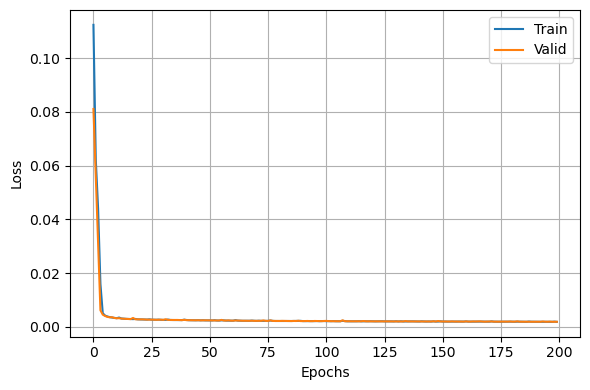
\includegraphics[width=0.45\linewidth]{figures/ae-loss.png}
    \caption{Loss function versus number of epochs.}
    \label{fig:ae-loss}
\end{figure}

\begin{figure}[H]
    \centering
    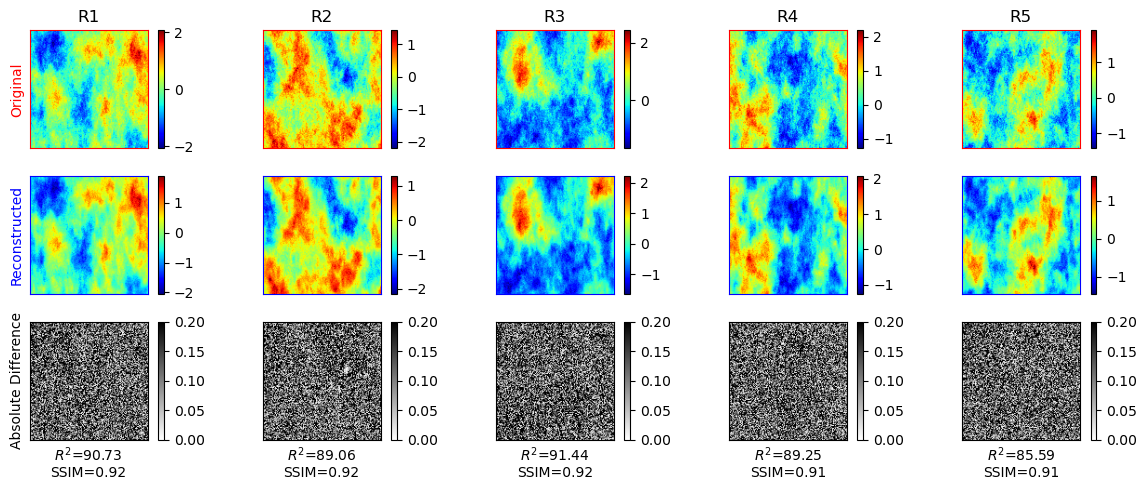
\includegraphics[width=\linewidth]{figures/ae-rec-best.png}
    \caption{Reconstructed image using latent dimension 256 in the AutoEncoder for the first 5 realizations (R1-R5). The bottom row shows the absolute difference, calculated using Eq.~\ref{eq:abserr}.}
    \label{fig:ae-rec-best}
\end{figure}

\pagebreak
%%% Conclusions %%%
\section*{Conclusions}
Dimensionality reduction techniques serve as powerful algorithms to project high-dimensional, complex datasets into lower dimensionality space while attempting to minimize the loss of information by extracting relevant patterns and features in the data. The latent representation, $z$, is designed to contain the most salient features of the data, and can be used as a proxy for complex and time-consuming routines such as reservoir simulation and history matching in the case of subsurface energy resource engineering.

Several dimensionality reduction algorithms were shown, namely singular value decomposition, principal component analysis, discrete wavelet transform, dictionary learning, and deep learning AutoEncoders. However, a much longer list of dimensionality reduction algorithms exists and can be useful for different types of datasets and applications. Table~\ref{tab:comparison} shows a comparison of the different dimensionality reduction techniques applied to the geologic uncertainty model dataset in terms of reconstruction accuracy and computational costs. Ultimately, the goal here is to obtain a compressed representation of the data that can be used to accelerate expensive computations, and the user must carefully select and design the dimensionality reduction algorithm according to the data needs. The tradeoff between compression and reconstruction accuracy is typically the main concern, as perfectly lossless compression is hard to obtain. Most engineering applications can benefit from slightly lossy compression at the benefit of significant computational acceleration.

\begin{table}[H]
    \centering
    \begin{tabular}{|l|l|l|l|l|l|}
    \hline
        & 20\% CR & 50\% CR & 80\% CR & 95\% CR & Time [s]  \\
    \hline
    SVD & 11  & 83  & 288 & 441 & 21.1          \\
    PCA & 2   & 8   & 36  & 234 & 2.6           \\
    DWT & 7   & 30  & 60  & 125 & 1.3           \\
    DL  & 16  & 191 & 426 & 491 & 94.6          \\
    \hline
    \end{tabular}
    \caption{Latent space dimension based on reconstruction accuracy. Four different dimensionality reduction techniques (SVD, PCA, DWT, DL) are compared based on different compression ratios (CR) (\emph{coefficients retained} / \emph{total number of features}) and their average CPU time required (in seconds) for compression and reconstruction.}
    \label{tab:comparison}
\end{table}

\pagebreak
%%%%% BACKMATTER %%%%%
\section*{Code Availability}
The code is publicly available on the authors GitHub repository: \\ https://github.com/misaelmmorales/Dimensionality-Reduction

\section*{Acknowledgments}
The authors thank the Formation Evaluation (FE) and Digital Reservoir Characterization Technology (DIRECT) Industry Affiliate Programs at the University of Texas at Austin for supporting this work.

\section*{Declaration of competing interest}
The authors declare that they have no known competing financial interests or personal relationships that could have appeared to influence the work reported in this paper.

%%%%% APPENDIX %%%%%
\pagebreak
\appendix

% SVD %
\section{Singular Value Decomposition (SVD) Code}\label{app:svd}
\inputminted[frame=lines, framesep=2mm, baselinestretch=1.2, 
             bgcolor=LightGray, fontsize=\footnotesize, linenos]
{python}{codes/svd.py}

% PCA %
\pagebreak
\section{Principal Component Analysis (PCA) Code}\label{app:pca}
\inputminted[frame=lines, framesep=2mm, baselinestretch=1.2, 
             bgcolor=LightGray, fontsize=\footnotesize, linenos]
{python}{codes/pca.py}

% DWT %
\pagebreak
\section{Discrete Wavelet Transform (DWT) Code}\label{app:dwt}
\inputminted[frame=lines, framesep=2mm, baselinestretch=1.2, 
             bgcolor=LightGray, fontsize=\footnotesize, linenos]
{python}{codes/dwt.py}

% DL %
\pagebreak
\section{Dictionary Learning (DL) Code}\label{app:dl}
\inputminted[frame=lines, framesep=2mm, baselinestretch=1.2, 
             bgcolor=LightGray, fontsize=\footnotesize, linenos]
{python}{codes/dl.py}

% AE %
\pagebreak
\section{AutoEncoder (AE) Code}\label{app:ae}
\inputminted[frame=lines, framesep=2mm, baselinestretch=1.2, 
             bgcolor=LightGray, fontsize=\footnotesize, linenos]
{python}{codes/ae.py}

%%% BIBLIOGRAPHY %%%
\pagebreak
\nolinenumbers
\bibliography{references}
\end{document}